\section{Recurrent Neural Networks}
\subsection*{Simple RNNs}
\term{Hidden state space sequence:} $\bs{h}^t=F(\bs{h}^{t-1},\bs{x}^t,\bs{\theta}), \; \bs{h}^0=\bs{0},t\leq s$ (Markov P. \& $F\bot t$)

\term{RNN:} $F(\bs{h},\bs{x};\bs{\theta})=\sigma(\bs{W}\bs{h}+\bs{U}\bs{x}+\bs{b})$

Optionally:
$\bs{y}=H(\bs{h};\bs{\theta}):=\sigma(\bs{V}\bs{h}+\bs{c})$

\subsection*{Sequence Loss Function}
\term{Settings:} 1. Normal $L$ for $\bs{h}^T\mapsto H(\bs{h}^T;\theta)=\bs{y}$

2. $\mathcal{R}(\bs{y}^1,\dots,\bs{y}^T)=\sum^T_{t=1} \mathcal{R}(\bs{y}^t)=\sum_{t} \mathcal{R}(H(\bs{h}^t;\theta))$

\begin{multicols}{2}
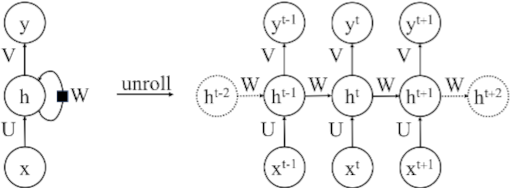
\includegraphics[width=\textwidth/8]{ETH-DS-2020/AML/Resources/unroll_rnn.png}

\term{Variable length noisy memory:} $(\bs{x}^1,\dots,\bs{x}^{t-1})\mapsto\bs{h}^t$
\end{multicols}
\term{Adv. over $T$-node f.c. layer:} param. sharing

\term{Backprop. through time:} $\dot{\sigma}_i^t:=\sigma'(\bar{F}(\bs{h}^{t-1},\bs{x}^t))$

$\frac{\partial\mathcal{R}}{\partial w_{ij}}=\sum^s_{t=1} \frac{\partial\mathcal{R}}{\partial \bs{h}^t_i}\cdot \frac{\partial\bs{h}^t_i}{\partial w_{ij}}=\sum^s_{t=1} \frac{\partial\mathcal{R}}{\partial \bs{h}^t_i}\cdot \dot{\sigma}_i^t \cdot \bs{h}^{t-1}_j$

$\frac{\partial\mathcal{R}}{\partial u_{ik}}=\sum^s_{t=1} \frac{\partial\mathcal{R}}{\partial \bs{h}^t_i}\cdot \frac{\partial\bs{h}^t_i}{\partial u_{ik}}=\sum^s_{t=1} \frac{\partial\mathcal{R}}{\partial \bs{h}^t_i}\cdot \dot{\sigma}_i^t \cdot \bs{x}^{t}_k$

\subsubsection*{$(\bs{y}=\bs{y}^s)$-RNNs/last step RNNs}

$\nabla_{\bs{h}^t} \mathcal{R} =[\prod^s_{r=t+1}\bs{W}^T \bs{S}(\bs{h}^r)]\cdot\bs{J}_H\cdot\nabla_{\bs{y}}\mathcal{R}$

$=[\prod^s_{r=t+1}\bs{W}^T \bs{S}(\bs{h}^r)]\cdot\bs{z},$
w $\bs{S}(\bs{h}^r)=\diag (\dot{\sigma}^r_1,\dots,\dot{\sigma}^r_n)$

$\leq \bs{I}$ for $\sigma\in\{\text{logistic, tanh, ReLu}\}$
\subsubsection*{Vanishing/Exploding Gradients w }
$\sigma_{\max}(\bs{W})<1,\; \bs{S}(\cdot)\leq \bs{I}\implies ||\nabla_{\bs{x}^t}\mathcal{R}||\stackrel{s-t\rightarrow \infty}{\rightarrow}0$

$\sigma_{\max}(\bs{J})>1 \implies$ ``gradients explode''

%$||\prod^s_{r=t+1}\bs{W}^T \bs{S}(\bs{h}^t)||_2
%\stackrel{\text{if }\bs{S}(\cdot)\leq \bs{I}}{\leq}
%||\prod^s_{r=t+1}\bs{W}^T||_2
%\leq
%||\bs{W}||^{s-t}_2
%\leq
%[\sigma_{\max}(\bs{W})^{s-t}]\stackrel{\text{if } \sigma(\bs{W})<1}{\rightarrow}0$ as $s-t\rightarrow \infty$

\begin{multicols}{2}
\term{Reverse order RNNs:}
$\bs{g}^t=G(\bs{x}^t,\bs{g}^{t+1};\bs{\theta})$\\
\term{Bi-directional RNNs:}
see pic (right)

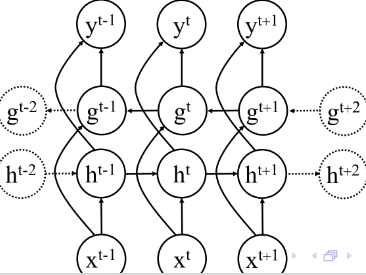
\includegraphics[width=\textwidth/11
]{ETH-DS-2020/AML/Resources/bi-directional.png}
\end{multicols}
\begin{multicols}{2}
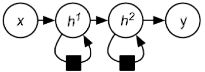
\includegraphics[width=\textwidth/9
]{ETH-DS-2020/AML/Resources/hierarchical2.png}

$\bs{h}^{t,l}=F(\bs{h}^{t-1,l},\bs{x}^{t};\bs{\theta}),\; (l=1,..,L),$ $\bs{y}^t=H(\bs{h}^{t,L};\bs{\theta})$
\end{multicols}
(-) Long term retention vs. short term changes

\subsection*{LSTM}
Forget gate: $\bs{f}_t=\sigma(\bs{W}_f\cdot[\bs{h}_{t-1},\bs{x}_t]+\bs{b}_f)$

Input gate: $\bs{i}_t=\sigma(\bs{W}_i\cdot[\bs{h}_{t-1},\bs{x}_t]+\bs{b}_i)$

Candidate: $\tilde{C}_t=\tanh(\bs{W}_C\cdot [\bs{h}_{t-1},\bs{x}_t]+\bs{b}_C)$

Cell: $\bs{C}_t=\bs{f}_t\odot \bs{C}_{t-1}+\bs{i}_t\odot\tilde{\bs{C}}_t$

Output: $\bs{o}_t= \sigma(\bs{W}_o\cdot[\bs{h}_{t-1},\bs{x}_t]+\bs{b}_o)$

Noisy memory: $\bs{h}_t=\bs{o}_t\odot \tanh(\bs{C}_t)$
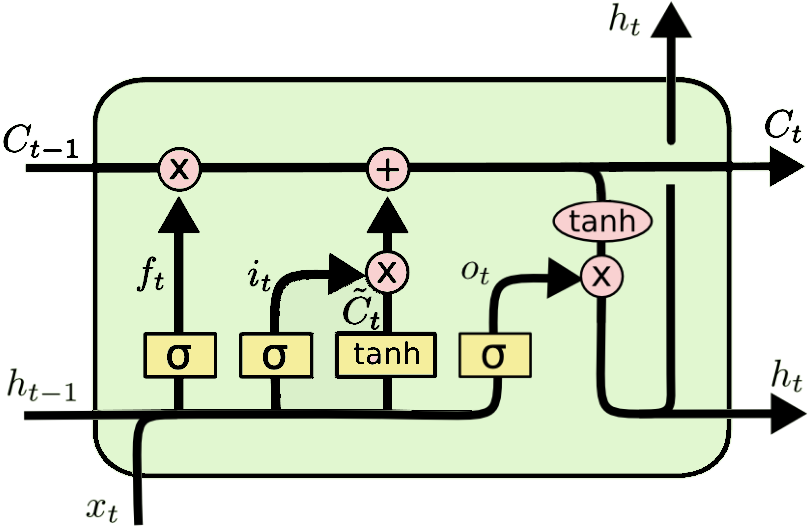
\includegraphics[width=\textwidth/5
]{ETH-DS-2020/AML/Resources/lstm_edited.png}
\subsection*{GRU}
\begin{multicols}{2}
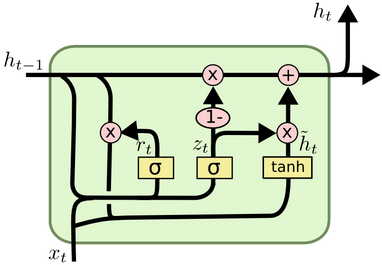
\includegraphics[width=\textwidth/8
]{ETH-DS-2020/AML/Resources/GRU.png}

$\bs{z}_t= \sigma(\bs{W}_z\cdot[\bs{h}_{t-1},\bs{x}_t])$

Remember gate: $\bs{r}_t= \sigma(\bs{W}_r\cdot[\bs{h}_{t-1},\bs{x}_t])$

$\tilde{\bs{h}}_t= \tanh(\bs{W}\cdot[\bs{r}_t\odot\bs{h}_{t-1},\bs{x}_t])$

ConvexOld+New: $\bs{h}_t=(1-\bs{z}_t)\odot\bs{h}_{t-1}
+\tilde{\bs{h}_t}\odot\bs{z}_t$
\end{multicols}

\subsection*{Unsegmented Sequences}
$p(\bs{\pi}|\overrightarrow{x})=\prod^T_{t=1}y_{\pi_t}$ w $\bs{\pi}_t$ label+blank distrib.

$p(\bs{l}|\overrightarrow{x})=\sum_{\pi\in B^{-1}(\bs{l})}p(\bs{\pi}|\overrightarrow{x})$

\subsection*{Learning Sequences}
Learn: $p(\bs{y}^{1:T}|\bs{x}^{1:T})\approx\prod^T_{t=1} p(\bs{y}^t|\bs{x}^{1:t},\bs{y}^{1:t-1})$

Naive RNN: $\bs{x}^{1:t}\stackrel{F}{\mapsto}\bs{h}^t, \bs{h}^t\stackrel{H}{\mapsto}\bs{\mu}^t, \bs{\mu}^t\mapsto p(\bs{y}^t)$

Problem: $p(\bs{y}^t)$ depends on $\bs{y}^{1:t-1}$ only thru $\bs{h}^t$

Cond. $\bot$ assumption: $p(\bs{y}^t|\bs{x}^t,\bs{y}^{1:t-1})=p(\bs{y}^t|\bs{x}^t)$


\begin{multicols}{2}
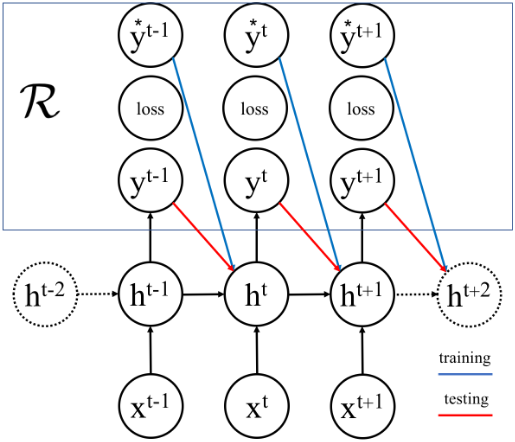
\includegraphics[width=\textwidth/7
]{ETH-DS-2020/AML/Resources/seq_feedback.png}
\term{Output feedback}\\
During train: Teacher forcing\\
(+): improves learn\\
(-): biased training\\
$\; \; \; \;$
\textcolor{red}{Seq2Seq:}\\
$\; \; \; \;$ Encoder-Decoder
\end{multicols}
\textcolor{purple}{Encoder:} $(\bs{x}^1,\dots,\bs{x}^T)\mapsto\bs{z}$ (e.g. RNN w $\bs{z}=\bs{h}^T$)

\color{purple}{Decoder:} $\bs{z}\mapsto(\bs{y}^1,\dots,\bs{y}^S)$ \color{myblue}
(e.g. RNN  output feedback and a stop symbol)

\term{ImageCapt:}Image Enc+Seq2SeqDec+Finetune